\documentclass{article} % For LaTeX2e
\usepackage{iclr2025_conference,times}

% Optional math commands from https://github.com/goodfeli/dlbook_notation.
%%%%% NEW MATH DEFINITIONS %%%%%

\usepackage{amsmath,amsfonts,bm}

% Mark sections of captions for referring to divisions of figures
\newcommand{\figleft}{{\em (Left)}}
\newcommand{\figcenter}{{\em (Center)}}
\newcommand{\figright}{{\em (Right)}}
\newcommand{\figtop}{{\em (Top)}}
\newcommand{\figbottom}{{\em (Bottom)}}
\newcommand{\captiona}{{\em (a)}}
\newcommand{\captionb}{{\em (b)}}
\newcommand{\captionc}{{\em (c)}}
\newcommand{\captiond}{{\em (d)}}

% Highlight a newly defined term
\newcommand{\newterm}[1]{{\bf #1}}


% Figure reference, lower-case.
\def\figref#1{figure~\ref{#1}}
% Figure reference, capital. For start of sentence
\def\Figref#1{Figure~\ref{#1}}
\def\twofigref#1#2{figures \ref{#1} and \ref{#2}}
\def\quadfigref#1#2#3#4{figures \ref{#1}, \ref{#2}, \ref{#3} and \ref{#4}}
% Section reference, lower-case.
\def\secref#1{section~\ref{#1}}
% Section reference, capital.
\def\Secref#1{Section~\ref{#1}}
% Reference to two sections.
\def\twosecrefs#1#2{sections \ref{#1} and \ref{#2}}
% Reference to three sections.
\def\secrefs#1#2#3{sections \ref{#1}, \ref{#2} and \ref{#3}}
% Reference to an equation, lower-case.
\def\eqref#1{equation~\ref{#1}}
% Reference to an equation, upper case
\def\Eqref#1{Equation~\ref{#1}}
% A raw reference to an equation---avoid using if possible
\def\plaineqref#1{\ref{#1}}
% Reference to a chapter, lower-case.
\def\chapref#1{chapter~\ref{#1}}
% Reference to an equation, upper case.
\def\Chapref#1{Chapter~\ref{#1}}
% Reference to a range of chapters
\def\rangechapref#1#2{chapters\ref{#1}--\ref{#2}}
% Reference to an algorithm, lower-case.
\def\algref#1{algorithm~\ref{#1}}
% Reference to an algorithm, upper case.
\def\Algref#1{Algorithm~\ref{#1}}
\def\twoalgref#1#2{algorithms \ref{#1} and \ref{#2}}
\def\Twoalgref#1#2{Algorithms \ref{#1} and \ref{#2}}
% Reference to a part, lower case
\def\partref#1{part~\ref{#1}}
% Reference to a part, upper case
\def\Partref#1{Part~\ref{#1}}
\def\twopartref#1#2{parts \ref{#1} and \ref{#2}}

\def\ceil#1{\lceil #1 \rceil}
\def\floor#1{\lfloor #1 \rfloor}
\def\1{\bm{1}}
\newcommand{\train}{\mathcal{D}}
\newcommand{\valid}{\mathcal{D_{\mathrm{valid}}}}
\newcommand{\test}{\mathcal{D_{\mathrm{test}}}}

\def\eps{{\epsilon}}


% Random variables
\def\reta{{\textnormal{$\eta$}}}
\def\ra{{\textnormal{a}}}
\def\rb{{\textnormal{b}}}
\def\rc{{\textnormal{c}}}
\def\rd{{\textnormal{d}}}
\def\re{{\textnormal{e}}}
\def\rf{{\textnormal{f}}}
\def\rg{{\textnormal{g}}}
\def\rh{{\textnormal{h}}}
\def\ri{{\textnormal{i}}}
\def\rj{{\textnormal{j}}}
\def\rk{{\textnormal{k}}}
\def\rl{{\textnormal{l}}}
% rm is already a command, just don't name any random variables m
\def\rn{{\textnormal{n}}}
\def\ro{{\textnormal{o}}}
\def\rp{{\textnormal{p}}}
\def\rq{{\textnormal{q}}}
\def\rr{{\textnormal{r}}}
\def\rs{{\textnormal{s}}}
\def\rt{{\textnormal{t}}}
\def\ru{{\textnormal{u}}}
\def\rv{{\textnormal{v}}}
\def\rw{{\textnormal{w}}}
\def\rx{{\textnormal{x}}}
\def\ry{{\textnormal{y}}}
\def\rz{{\textnormal{z}}}

% Random vectors
\def\rvepsilon{{\mathbf{\epsilon}}}
\def\rvtheta{{\mathbf{\theta}}}
\def\rva{{\mathbf{a}}}
\def\rvb{{\mathbf{b}}}
\def\rvc{{\mathbf{c}}}
\def\rvd{{\mathbf{d}}}
\def\rve{{\mathbf{e}}}
\def\rvf{{\mathbf{f}}}
\def\rvg{{\mathbf{g}}}
\def\rvh{{\mathbf{h}}}
\def\rvu{{\mathbf{i}}}
\def\rvj{{\mathbf{j}}}
\def\rvk{{\mathbf{k}}}
\def\rvl{{\mathbf{l}}}
\def\rvm{{\mathbf{m}}}
\def\rvn{{\mathbf{n}}}
\def\rvo{{\mathbf{o}}}
\def\rvp{{\mathbf{p}}}
\def\rvq{{\mathbf{q}}}
\def\rvr{{\mathbf{r}}}
\def\rvs{{\mathbf{s}}}
\def\rvt{{\mathbf{t}}}
\def\rvu{{\mathbf{u}}}
\def\rvv{{\mathbf{v}}}
\def\rvw{{\mathbf{w}}}
\def\rvx{{\mathbf{x}}}
\def\rvy{{\mathbf{y}}}
\def\rvz{{\mathbf{z}}}

% Elements of random vectors
\def\erva{{\textnormal{a}}}
\def\ervb{{\textnormal{b}}}
\def\ervc{{\textnormal{c}}}
\def\ervd{{\textnormal{d}}}
\def\erve{{\textnormal{e}}}
\def\ervf{{\textnormal{f}}}
\def\ervg{{\textnormal{g}}}
\def\ervh{{\textnormal{h}}}
\def\ervi{{\textnormal{i}}}
\def\ervj{{\textnormal{j}}}
\def\ervk{{\textnormal{k}}}
\def\ervl{{\textnormal{l}}}
\def\ervm{{\textnormal{m}}}
\def\ervn{{\textnormal{n}}}
\def\ervo{{\textnormal{o}}}
\def\ervp{{\textnormal{p}}}
\def\ervq{{\textnormal{q}}}
\def\ervr{{\textnormal{r}}}
\def\ervs{{\textnormal{s}}}
\def\ervt{{\textnormal{t}}}
\def\ervu{{\textnormal{u}}}
\def\ervv{{\textnormal{v}}}
\def\ervw{{\textnormal{w}}}
\def\ervx{{\textnormal{x}}}
\def\ervy{{\textnormal{y}}}
\def\ervz{{\textnormal{z}}}

% Random matrices
\def\rmA{{\mathbf{A}}}
\def\rmB{{\mathbf{B}}}
\def\rmC{{\mathbf{C}}}
\def\rmD{{\mathbf{D}}}
\def\rmE{{\mathbf{E}}}
\def\rmF{{\mathbf{F}}}
\def\rmG{{\mathbf{G}}}
\def\rmH{{\mathbf{H}}}
\def\rmI{{\mathbf{I}}}
\def\rmJ{{\mathbf{J}}}
\def\rmK{{\mathbf{K}}}
\def\rmL{{\mathbf{L}}}
\def\rmM{{\mathbf{M}}}
\def\rmN{{\mathbf{N}}}
\def\rmO{{\mathbf{O}}}
\def\rmP{{\mathbf{P}}}
\def\rmQ{{\mathbf{Q}}}
\def\rmR{{\mathbf{R}}}
\def\rmS{{\mathbf{S}}}
\def\rmT{{\mathbf{T}}}
\def\rmU{{\mathbf{U}}}
\def\rmV{{\mathbf{V}}}
\def\rmW{{\mathbf{W}}}
\def\rmX{{\mathbf{X}}}
\def\rmY{{\mathbf{Y}}}
\def\rmZ{{\mathbf{Z}}}

% Elements of random matrices
\def\ermA{{\textnormal{A}}}
\def\ermB{{\textnormal{B}}}
\def\ermC{{\textnormal{C}}}
\def\ermD{{\textnormal{D}}}
\def\ermE{{\textnormal{E}}}
\def\ermF{{\textnormal{F}}}
\def\ermG{{\textnormal{G}}}
\def\ermH{{\textnormal{H}}}
\def\ermI{{\textnormal{I}}}
\def\ermJ{{\textnormal{J}}}
\def\ermK{{\textnormal{K}}}
\def\ermL{{\textnormal{L}}}
\def\ermM{{\textnormal{M}}}
\def\ermN{{\textnormal{N}}}
\def\ermO{{\textnormal{O}}}
\def\ermP{{\textnormal{P}}}
\def\ermQ{{\textnormal{Q}}}
\def\ermR{{\textnormal{R}}}
\def\ermS{{\textnormal{S}}}
\def\ermT{{\textnormal{T}}}
\def\ermU{{\textnormal{U}}}
\def\ermV{{\textnormal{V}}}
\def\ermW{{\textnormal{W}}}
\def\ermX{{\textnormal{X}}}
\def\ermY{{\textnormal{Y}}}
\def\ermZ{{\textnormal{Z}}}

% Vectors
\def\vzero{{\bm{0}}}
\def\vone{{\bm{1}}}
\def\vmu{{\bm{\mu}}}
\def\vtheta{{\bm{\theta}}}
\def\va{{\bm{a}}}
\def\vb{{\bm{b}}}
\def\vc{{\bm{c}}}
\def\vd{{\bm{d}}}
\def\ve{{\bm{e}}}
\def\vf{{\bm{f}}}
\def\vg{{\bm{g}}}
\def\vh{{\bm{h}}}
\def\vi{{\bm{i}}}
\def\vj{{\bm{j}}}
\def\vk{{\bm{k}}}
\def\vl{{\bm{l}}}
\def\vm{{\bm{m}}}
\def\vn{{\bm{n}}}
\def\vo{{\bm{o}}}
\def\vp{{\bm{p}}}
\def\vq{{\bm{q}}}
\def\vr{{\bm{r}}}
\def\vs{{\bm{s}}}
\def\vt{{\bm{t}}}
\def\vu{{\bm{u}}}
\def\vv{{\bm{v}}}
\def\vw{{\bm{w}}}
\def\vx{{\bm{x}}}
\def\vy{{\bm{y}}}
\def\vz{{\bm{z}}}

% Elements of vectors
\def\evalpha{{\alpha}}
\def\evbeta{{\beta}}
\def\evepsilon{{\epsilon}}
\def\evlambda{{\lambda}}
\def\evomega{{\omega}}
\def\evmu{{\mu}}
\def\evpsi{{\psi}}
\def\evsigma{{\sigma}}
\def\evtheta{{\theta}}
\def\eva{{a}}
\def\evb{{b}}
\def\evc{{c}}
\def\evd{{d}}
\def\eve{{e}}
\def\evf{{f}}
\def\evg{{g}}
\def\evh{{h}}
\def\evi{{i}}
\def\evj{{j}}
\def\evk{{k}}
\def\evl{{l}}
\def\evm{{m}}
\def\evn{{n}}
\def\evo{{o}}
\def\evp{{p}}
\def\evq{{q}}
\def\evr{{r}}
\def\evs{{s}}
\def\evt{{t}}
\def\evu{{u}}
\def\evv{{v}}
\def\evw{{w}}
\def\evx{{x}}
\def\evy{{y}}
\def\evz{{z}}

% Matrix
\def\mA{{\bm{A}}}
\def\mB{{\bm{B}}}
\def\mC{{\bm{C}}}
\def\mD{{\bm{D}}}
\def\mE{{\bm{E}}}
\def\mF{{\bm{F}}}
\def\mG{{\bm{G}}}
\def\mH{{\bm{H}}}
\def\mI{{\bm{I}}}
\def\mJ{{\bm{J}}}
\def\mK{{\bm{K}}}
\def\mL{{\bm{L}}}
\def\mM{{\bm{M}}}
\def\mN{{\bm{N}}}
\def\mO{{\bm{O}}}
\def\mP{{\bm{P}}}
\def\mQ{{\bm{Q}}}
\def\mR{{\bm{R}}}
\def\mS{{\bm{S}}}
\def\mT{{\bm{T}}}
\def\mU{{\bm{U}}}
\def\mV{{\bm{V}}}
\def\mW{{\bm{W}}}
\def\mX{{\bm{X}}}
\def\mY{{\bm{Y}}}
\def\mZ{{\bm{Z}}}
\def\mBeta{{\bm{\beta}}}
\def\mPhi{{\bm{\Phi}}}
\def\mLambda{{\bm{\Lambda}}}
\def\mSigma{{\bm{\Sigma}}}

% Tensor
\DeclareMathAlphabet{\mathsfit}{\encodingdefault}{\sfdefault}{m}{sl}
\SetMathAlphabet{\mathsfit}{bold}{\encodingdefault}{\sfdefault}{bx}{n}
\newcommand{\tens}[1]{\bm{\mathsfit{#1}}}
\def\tA{{\tens{A}}}
\def\tB{{\tens{B}}}
\def\tC{{\tens{C}}}
\def\tD{{\tens{D}}}
\def\tE{{\tens{E}}}
\def\tF{{\tens{F}}}
\def\tG{{\tens{G}}}
\def\tH{{\tens{H}}}
\def\tI{{\tens{I}}}
\def\tJ{{\tens{J}}}
\def\tK{{\tens{K}}}
\def\tL{{\tens{L}}}
\def\tM{{\tens{M}}}
\def\tN{{\tens{N}}}
\def\tO{{\tens{O}}}
\def\tP{{\tens{P}}}
\def\tQ{{\tens{Q}}}
\def\tR{{\tens{R}}}
\def\tS{{\tens{S}}}
\def\tT{{\tens{T}}}
\def\tU{{\tens{U}}}
\def\tV{{\tens{V}}}
\def\tW{{\tens{W}}}
\def\tX{{\tens{X}}}
\def\tY{{\tens{Y}}}
\def\tZ{{\tens{Z}}}


% Graph
\def\gA{{\mathcal{A}}}
\def\gB{{\mathcal{B}}}
\def\gC{{\mathcal{C}}}
\def\gD{{\mathcal{D}}}
\def\gE{{\mathcal{E}}}
\def\gF{{\mathcal{F}}}
\def\gG{{\mathcal{G}}}
\def\gH{{\mathcal{H}}}
\def\gI{{\mathcal{I}}}
\def\gJ{{\mathcal{J}}}
\def\gK{{\mathcal{K}}}
\def\gL{{\mathcal{L}}}
\def\gM{{\mathcal{M}}}
\def\gN{{\mathcal{N}}}
\def\gO{{\mathcal{O}}}
\def\gP{{\mathcal{P}}}
\def\gQ{{\mathcal{Q}}}
\def\gR{{\mathcal{R}}}
\def\gS{{\mathcal{S}}}
\def\gT{{\mathcal{T}}}
\def\gU{{\mathcal{U}}}
\def\gV{{\mathcal{V}}}
\def\gW{{\mathcal{W}}}
\def\gX{{\mathcal{X}}}
\def\gY{{\mathcal{Y}}}
\def\gZ{{\mathcal{Z}}}

% Sets
\def\sA{{\mathbb{A}}}
\def\sB{{\mathbb{B}}}
\def\sC{{\mathbb{C}}}
\def\sD{{\mathbb{D}}}
% Don't use a set called E, because this would be the same as our symbol
% for expectation.
\def\sF{{\mathbb{F}}}
\def\sG{{\mathbb{G}}}
\def\sH{{\mathbb{H}}}
\def\sI{{\mathbb{I}}}
\def\sJ{{\mathbb{J}}}
\def\sK{{\mathbb{K}}}
\def\sL{{\mathbb{L}}}
\def\sM{{\mathbb{M}}}
\def\sN{{\mathbb{N}}}
\def\sO{{\mathbb{O}}}
\def\sP{{\mathbb{P}}}
\def\sQ{{\mathbb{Q}}}
\def\sR{{\mathbb{R}}}
\def\sS{{\mathbb{S}}}
\def\sT{{\mathbb{T}}}
\def\sU{{\mathbb{U}}}
\def\sV{{\mathbb{V}}}
\def\sW{{\mathbb{W}}}
\def\sX{{\mathbb{X}}}
\def\sY{{\mathbb{Y}}}
\def\sZ{{\mathbb{Z}}}

% Entries of a matrix
\def\emLambda{{\Lambda}}
\def\emA{{A}}
\def\emB{{B}}
\def\emC{{C}}
\def\emD{{D}}
\def\emE{{E}}
\def\emF{{F}}
\def\emG{{G}}
\def\emH{{H}}
\def\emI{{I}}
\def\emJ{{J}}
\def\emK{{K}}
\def\emL{{L}}
\def\emM{{M}}
\def\emN{{N}}
\def\emO{{O}}
\def\emP{{P}}
\def\emQ{{Q}}
\def\emR{{R}}
\def\emS{{S}}
\def\emT{{T}}
\def\emU{{U}}
\def\emV{{V}}
\def\emW{{W}}
\def\emX{{X}}
\def\emY{{Y}}
\def\emZ{{Z}}
\def\emSigma{{\Sigma}}

% entries of a tensor
% Same font as tensor, without \bm wrapper
\newcommand{\etens}[1]{\mathsfit{#1}}
\def\etLambda{{\etens{\Lambda}}}
\def\etA{{\etens{A}}}
\def\etB{{\etens{B}}}
\def\etC{{\etens{C}}}
\def\etD{{\etens{D}}}
\def\etE{{\etens{E}}}
\def\etF{{\etens{F}}}
\def\etG{{\etens{G}}}
\def\etH{{\etens{H}}}
\def\etI{{\etens{I}}}
\def\etJ{{\etens{J}}}
\def\etK{{\etens{K}}}
\def\etL{{\etens{L}}}
\def\etM{{\etens{M}}}
\def\etN{{\etens{N}}}
\def\etO{{\etens{O}}}
\def\etP{{\etens{P}}}
\def\etQ{{\etens{Q}}}
\def\etR{{\etens{R}}}
\def\etS{{\etens{S}}}
\def\etT{{\etens{T}}}
\def\etU{{\etens{U}}}
\def\etV{{\etens{V}}}
\def\etW{{\etens{W}}}
\def\etX{{\etens{X}}}
\def\etY{{\etens{Y}}}
\def\etZ{{\etens{Z}}}

% The true underlying data generating distribution
\newcommand{\pdata}{p_{\rm{data}}}
% The empirical distribution defined by the training set
\newcommand{\ptrain}{\hat{p}_{\rm{data}}}
\newcommand{\Ptrain}{\hat{P}_{\rm{data}}}
% The model distribution
\newcommand{\pmodel}{p_{\rm{model}}}
\newcommand{\Pmodel}{P_{\rm{model}}}
\newcommand{\ptildemodel}{\tilde{p}_{\rm{model}}}
% Stochastic autoencoder distributions
\newcommand{\pencode}{p_{\rm{encoder}}}
\newcommand{\pdecode}{p_{\rm{decoder}}}
\newcommand{\precons}{p_{\rm{reconstruct}}}

\newcommand{\laplace}{\mathrm{Laplace}} % Laplace distribution

\newcommand{\E}{\mathbb{E}}
\newcommand{\Ls}{\mathcal{L}}
\newcommand{\R}{\mathbb{R}}
\newcommand{\emp}{\tilde{p}}
\newcommand{\lr}{\alpha}
\newcommand{\reg}{\lambda}
\newcommand{\rect}{\mathrm{rectifier}}
\newcommand{\softmax}{\mathrm{softmax}}
\newcommand{\sigmoid}{\sigma}
\newcommand{\softplus}{\zeta}
\newcommand{\KL}{D_{\mathrm{KL}}}
\newcommand{\Var}{\mathrm{Var}}
\newcommand{\standarderror}{\mathrm{SE}}
\newcommand{\Cov}{\mathrm{Cov}}
% Wolfram Mathworld says $L^2$ is for function spaces and $\ell^2$ is for vectors
% But then they seem to use $L^2$ for vectors throughout the site, and so does
% wikipedia.
\newcommand{\normlzero}{L^0}
\newcommand{\normlone}{L^1}
\newcommand{\normltwo}{L^2}
\newcommand{\normlp}{L^p}
\newcommand{\normmax}{L^\infty}

\newcommand{\parents}{Pa} % See usage in notation.tex. Chosen to match Daphne's book.

\DeclareMathOperator*{\argmax}{arg\,max}
\DeclareMathOperator*{\argmin}{arg\,min}

\DeclareMathOperator{\sign}{sign}
\DeclareMathOperator{\Tr}{Tr}
\let\ab\allowbreak


\usepackage{hyperref}
\usepackage{url}
\usepackage{booktabs}
\usepackage{graphicx}
\usepackage{amsmath}
\usepackage{amssymb}
\usepackage{multirow}
\usepackage[capitalize]{cleveref}

%%%%%%%%% TITLE - PLEASE UPDATE TITLE HERE
\title{How Flexible Must an AI Data Center Be? \\ SLO-Grounded Flexibility, Network-Aware Signals, and Certified Interconnection Maps}

\author{Ambitious AI Researcher\\
AI Research Institute\\
123 AI Avenue, ML City\\
\texttt{researcher@institute.ai}
}

\newcommand{\fix}{\marginpar{FIX}}
\newcommand{\new}{\marginpar{NEW}}

\begin{document}

\maketitle

\begin{abstract}
%%%%%%%%% ABSTRACT %%%%%%%%%
Large AI inference campuses are joining power grids faster than transmission can be built, and flexible interconnection is increasingly proposed as the remedy. Yet the flexibility of such campuses is usually assumed rather than derived, and it is evaluated against price or carbon signals that ignore the network. We close this gap end to end. First, we derive the grid-facing flexibility of a large language model (LLM) inference fleet from first principles. An iteration-level serving simulator, driven by a public production trace, turns p99 latency service-level objectives (SLOs) into a linear hourly envelope of firm power, power sheddable by GPU power capping, and deferrable batch energy with deadlines. Within the SLO, interactive serving can shed only 4.9\% of facility load; deferrable batch work, at 19.8\% of energy in our default setting, supplies most of the flexibility. Second, embedding this envelope in a year of network-constrained multi-period DC optimal power flow on the RTS-GMLC test system shows that the steering signal matters more than the flexibility itself. With an identical envelope, following locational marginal emissions cuts the campus's hosting emissions by 5.7--12.3\%, whereas cost-optimal co-optimisation cuts them by 2.4--3.2\% and, at a coal-margined bus, raises them while lowering cost. Third, we compute a certified flexible-interconnection map. Power capping plus a few hours of deferral lets a 500\,MW campus connect without load shedding at 48 instead of 36 of 73 buses, raising hosting capacity from 35.25 to 42.90\,GW (+22\%). Finally, we find that end-to-end hard-constraint learners are either infeasible or far from optimal on this problem, for a structural reason we call the interior-anchor barrier, whereas exact constraint screening reaches the optimum with zero violations at 3.2$\times$ the speed of a full LP solve.
%%%%%%%%% ABSTRACT %%%%%%%%%
\end{abstract}

\section{Introduction}
\label{sec:intro}
%%%%%%%%% INTRODUCTION %%%%%%%%%
Data centers are among the fastest-growing electricity loads, and AI workloads are driving much of that growth \citep{masanet2020recalibrating,shehabi2024report,wu2022sustainable}. New campuses now request 100\,MW to 1\,GW connections, and interconnection queues and local transmission limits increasingly decide where and when they can be built. A widely discussed remedy is \emph{flexible interconnection}: a campus that can reduce or shift its consumption on request could connect at locations the grid could not otherwise serve. Data-center demand response has long been proposed as a grid resource \citep{wierman2014opportunities}, and carbon-aware computing shifts work in time and space to cleaner hours and places \citep{radovanovic2023carbon,wiesner2021letswait,hanafy2024carbonscaler}. Machine learning for power systems is a central theme of climate-focused ML research \citep{rolnick2022tackling}.

Three pieces are missing for AI inference campuses. \textbf{(i) Flexibility is assumed, not derived.} Grid studies typically posit that some fraction of a data center's load is shiftable or sheddable. For an LLM inference fleet, flexibility is bounded by p99 latency SLOs, namely time-to-first-token (TTFT) and time-per-output-token (TPOT), and by how much deferrable batch work exists. Serving-system research optimises energy and latency inside the cluster \citep{kwon2023pagedattention,patel2024splitwise,stojkovic2025dynamollm,you2023zeus}, but it does not produce the grid-facing envelope a system operator needs. \textbf{(ii) The grid is a signal, not a network.} Most flexibility studies follow price or average-carbon signals. Economic analysis shows that price-following flexible data centers can lower costs while raising emissions \citep{knittel2025flexible}, and locational marginal emissions have been proposed to guide geographic load shifting \citep{lindberg2021environmental,zhang2022remunerating}. Without transmission constraints, however, one cannot say \emph{where} a campus can connect, nor \emph{which} signal should steer it once congestion and locational marginal units are considered. \textbf{(iii) Fast solvers with hard guarantees are needed but untested at this scale.} Learning-to-optimise methods that enforce hard constraints promise fast feasible solutions \citep{donti2021dc3,tabas2022safe,liang2023homeomorphic}, yet joint fleet--grid dispatch is a multi-period LP with deadlines and load-shedding slack, where their behaviour is unknown.

We address all three on a public test system (RTS-GMLC; \citealp{barrows2020rts}) and a public production LLM trace \citep{stojkovic2025dynamollm}. Our contributions are:
\begin{itemize}
    \item \textbf{SLO-grounded flexibility envelopes.} An iteration-level serving simulator with a physically consistent power-cap model turns p99 SLOs into a \emph{linear} hourly envelope that plugs exactly into DC optimal power flow (\cref{sec:envelope}). Interactive serving is barely flexible (4.9\% of load sheddable); real flexibility comes from deferrable batch work.
    \item \textbf{Signals matter more than flexibility.} In a full year of network-constrained dispatch, the same envelope steered by locational marginal emissions (LMEs) cuts hosting emissions 3--4$\times$ more than cost co-optimisation. The ``lower cost, higher emissions'' effect appears exactly where coal is on the margin, and a carbon price aligns all signals (\cref{sec:exp_signals}).
    \item \textbf{A certified flexible-interconnection map.} For every bus and four campus sizes, we compute the minimum SLO-feasible flexibility needed to connect without load shedding. Stress-day screening is followed by full-year verification, and every solve is exact (\cref{sec:map,sec:exp_map}). Modest flexibility raises hosting capacity by 22\%.
    \item \textbf{The interior-anchor barrier.} We show why end-to-end hard-constraint learners struggle on OPF with value-of-lost-load slack, and that exact constraint screening is the practical route to fast, certifiably optimal solutions on this problem (\cref{sec:exp_solvers}).
\end{itemize}
%%%%%%%%% INTRODUCTION %%%%%%%%%

\section{Related Work}
\label{sec:related_work}
%%%%%%%%% RELATED WORK %%%%%%%%%
\paragraph{Data-center flexibility and carbon-aware load shifting.} Data-center demand response has been studied as a grid resource for over a decade \citep{wierman2014opportunities}. Carbon-aware computing shifts flexible work across hours and sites: Google's carbon-intelligent computing platform \citep{radovanovic2023carbon}, temporal workload shifting in the cloud \citep{wiesner2021letswait}, and elasticity-based carbon scaling \citep{hanafy2024carbonscaler}. These works treat the grid as an exogenous signal. \citet{lindberg2021environmental} use locational marginal CO$_2$ emissions from optimal power flow to guide geographic load shifting, and \citet{zhang2022remunerating} analyse how space--time load-shifting flexibility of data centers should be remunerated in electricity markets. \citet{knittel2025flexible} show that flexible data centers can lower costs yet raise emissions. Across this literature, flexibility is a parameter (a shiftable fraction) rather than a quantity derived from serving SLOs, and the question of \emph{where} a campus can be hosted is not addressed. We derive the envelope from serving physics and evaluate it inside network-constrained dispatch, including hosting maps. Our LME computation follows the standard marginal-unit analysis of constrained networks \citep{ruiz2010marginal}.

\paragraph{LLM inference serving and energy.} Modern LLM serving uses continuous batching \citep{yu2022orca}, paged KV-cache management \citep{kwon2023pagedattention} and chunked prefill to balance throughput and latency \citep{agrawal2024sarathi}. Splitwise separates prefill and decode phases \citep{patel2024splitwise}. DynamoLLM reconfigures inference clusters for energy efficiency under SLOs \citep{stojkovic2025dynamollm}, and power-management studies show that LLM inference tolerates power capping and oversubscription \citep{patel2024characterizing}. GPU energy can be traded against performance through power limits \citep{you2023zeus}. These systems optimise the cluster; we translate the same physics into a grid-facing linear envelope. Our timing model uses roofline reasoning \citep{williams2009roofline}.

\paragraph{Learning to optimise with hard constraints.} DC3 completes equality constraints and corrects inequality violations with unrolled gradient steps \citep{donti2021dc3}. Gauge maps \citep{tabas2022safe,li2023loop} and homeomorphic projection \citep{liang2023homeomorphic} map network outputs into a convex feasible set around an interior point. Differentiable projections enforce feasibility for energy-optimisation policies \citep{chen2021enforcing}, and FSNet adds a feasibility-seeking step \citep{nguyen2025fsnet}. For OPF specifically, DeepOPF \citep{pan2021deepopf} and learned AC-OPF solvers \citep{zamzam2020learning} predict dispatch directly, and data-driven constraint screening removes inactive network constraints \citep{pineda2020screening}. Decision-focused learning couples prediction and optimisation \citep{donti2017taskbased}. We identify a structural obstacle for interior-point-based guarantees in OPF with load-shedding slack, and we find that exact screening is the effective approach on our problem.
%%%%%%%%% RELATED WORK %%%%%%%%%

\section{Methodology}
\label{sec:method}
%%%%%%%%% METHOD %%%%%%%%%
\subsection{SLO-grounded flexibility envelopes}
\label{sec:envelope}
\paragraph{Replica model.} One replica is an 8-GPU server serving a 70B-class model with tensor parallelism. We simulate it at iteration level with chunked-prefill continuous batching: each iteration serves one decode token for every running sequence and fills the rest of a 2,048-token budget with prompt chunks \citep{agrawal2024sarathi,kwon2023pagedattention}. Iteration time follows a roofline model \citep{williams2009roofline}: prefill is compute-bound, and decode is bandwidth-bound, reading the weights and the KV cache once per step. Power capping is modelled consistently with timing. A phase demanding GPU power $P^{\mathrm{dem}} = P^{\mathrm{idle}} + (P^{\mathrm{TDP}} - P^{\mathrm{idle}})\,a$ under a cap $\kappa P^{\mathrm{TDP}} < P^{\mathrm{dem}}$ runs at relative performance
\begin{equation}
    \rho(\kappa) = \left(\frac{\kappa P^{\mathrm{TDP}} - P^{\mathrm{idle}}}{P^{\mathrm{dem}} - P^{\mathrm{idle}}}\right)^{\gamma},
    \label{eq:cap}
\end{equation}
with $\gamma = 1/3$ for compute-bound prefill and $\gamma = 0.15$ for memory-bound decode. For each service and cap $\kappa$, we find by bisection the largest Poisson request rate $\mu(\kappa)$ at which p99 TTFT and p99 TPOT meet the SLO.

\paragraph{Facility envelope.} For a facility of rated power $\bar P$, interactive replicas are provisioned each hour for the peak-minute load at 80\% of their full-power SLO capacity, and spare servers are kept in hot standby. Let $f_t$ be firm power (interactive serving at full power plus idle spares), $s_t$ the power shed by capping active replicas to the lowest cap whose SLO capacity still covers the peak-minute load, and $b_t$ the power drawn by deferrable batch work. With batch arrivals $A_t$ and deadline $D$, the facility draws
\begin{equation}
    d_t = f_t - s_t + b_t, \quad 0 \le s_t \le \bar s_t,\ \ \sum_{t \in \text{day}} s_t \le H \max_t \bar s_t, \quad 0 \le b_t \le \bar b_t,
    \label{eq:envelope}
\end{equation}
\begin{equation}
    \sum_{\tau \le t - D} A_\tau \;\le\; \sum_{\tau \le t} b_\tau \;\le\; \sum_{\tau \le t} A_\tau ,
    \label{eq:deadline}
\end{equation}
where $\bar s_t$ is the sheddable power, $H$ the daily capping budget (4 full-depth hours), and $\bar b_t$ the headroom of spare servers running batch work at the most energy-efficient cap. All constraints are linear, so the SLOs enter optimal power flow exactly. The \emph{inflexible} reference serves batch work as soon as capacity allows and never sheds.

\subsection{Network-constrained joint dispatch}
\label{sec:dispatch}
We solve multi-period DC optimal power flow in PTDF form with generator ramps, renewable curtailment, involuntary load shedding at a value of lost load (VOLL) of \$10{,}000/MWh, and the envelope \cref{eq:envelope,eq:deadline}, using HiGHS \citep{huangfu2018highs}. Locational marginal prices and locational marginal emissions are row marginals at the optimal basis: with $B$ the basis matrix, $y = B^{-\top} c_B$ with $c$ the cost vector gives the LMPs, and replacing $c$ by generator CO$_2$ rates gives the LMEs \citep{ruiz2010marginal}. A 48-hour-lookahead rolling horizon commits 24 hours per day and carries ramp state and the actual batch backlog. We compare operating modes that share one envelope: \emph{inflexible}; \emph{price-following}, \emph{average-carbon-following} and \emph{LME-following}, where the facility best-responds to the day-ahead signal at its bus taken from the inflexible run and the grid then re-dispatches; and \emph{co-optimised}, where the envelope sits inside the OPF. True emissions always come from the re-dispatch.

\subsection{Certified flexible-interconnection map}
\label{sec:map}
A campus of size $S$ at bus $n$ is \emph{hostable at level} $\ell$ if, with the operator co-optimising its level-$\ell$ envelope, the grid serves it with no involuntary load shedding and no missed batch deadline. The ladder keeps fleet, traffic and energy fixed and changes only what may move: L0 inflexible; L1 power capping within the SLO; L2/L3/L4 batch deferral with 4/12/24\,h deadlines; L5 capping down to a 2$\times$-relaxed SLO. We certify the minimum level in two stages, solving every instance exactly with screened HiGHS. \emph{Stage 1} solves 48 stress days (four per month, each a 48\,h window) and searches levels upward. A failure on a real day makes ``not hostable'' exact and makes the level below the reported minimum exactly infeasible. \emph{Stage 2} re-checks every flexible entry over all 365 days and raises it until every day passes.

\subsection{Solvers for the joint problem}
\label{sec:solvers}
We pose the 24\,h joint problem at one bus as a differentiable LP family. Free variables are rescaled to boxes; equalities are completed by the facility power and a \emph{distributed slack} that moves every generator by the same fraction of its range. We compare: DC3-style completion and correction \citep{donti2021dc3}; a gauge map \citep{tabas2022safe,li2023loop} around a closed-form strictly interior anchor; predict--correct--project, a closed-form ray projection in the spirit of homeomorphic projection \citep{liang2023homeomorphic}; FSNet-style feasibility seeking \citep{nguyen2025fsnet}; and exact line-constraint screening with constraint generation, using frequency-based or learned screens \citep{pineda2020screening}.
%%%%%%%%% METHOD %%%%%%%%%

\section{Experiments}
\label{sec:experiments}
%%%%%%%%% EXPERIMENTS %%%%%%%%%
\subsection{Setup}
\paragraph{Grid.} RTS-GMLC \citep{barrows2020rts}: 73 buses in 3 areas, 120 lines and 153 modelled generators, with 2020 hourly day-ahead load, wind, solar and hydro. Linear costs and CO$_2$ rates come from heat-rate curves; there is no unit commitment. Lines are derated to 0.6$\times$ nameplate to create a congested case. Without a data center, this case has 22{,}328 binding line-hours per year (4{,}114 at nameplate), a mean LME of 0.725\,t/MWh against an average emission rate of 0.446\,t/MWh, and \$104.8M of congestion rent. Coal steam units (\$22.9/MWh, 1.03\,t/MWh) undercut combined-cycle gas (\$29.0/MWh, 0.40\,t/MWh).
\paragraph{Workload and fleet.} We use the Azure LLM inference trace 2024 \citep{stojkovic2025dynamollm}: one week each of code-assistant (16.8M requests) and conversation (27.3M requests) traffic. Replicas are 8$\times$H100 (700\,W TDP); SLOs are p99 TTFT $\le$ 1\,s and p99 TPOT $\le$ 100\,ms; PUE is 1.2. By default, batch work fills 50\% of spare capacity. The default facility is rated at 300\,MW (30{,}864 servers). Fleet parameters not taken from datasheets are documented assumptions.
\paragraph{Sites.} Bus 101 (coal-heavy area 1), 122 (wind, area 1), 207 (radial pocket, area 2), 303 (wind pocket, area 3) and 313 (load centre, area 3).

\subsection{How flexible is an inference fleet?}
\label{sec:exp_envelope}
\Cref{fig:cap} shows the power--latency trade-off per replica. Capping to 70\% of TDP keeps 86.5\% (conversation) and 88.2\% (code) of the uncapped SLO capacity, above the 80\% provisioning level. At 60\% TDP, capacity collapses to 41.8\% and 20.1\%, because the chunked-prefill TPOT floor then exceeds 100\,ms. At nominal load, capping to 70\% lowers conversation server power from 6.51 to 5.68\,kW. For batch work, where latency is unconstrained, deeper caps are \emph{more} efficient: energy falls from 6.02\,J/token uncapped to 4.60\,J/token at a 50\% cap.

\begin{figure}[t]
    \centering
    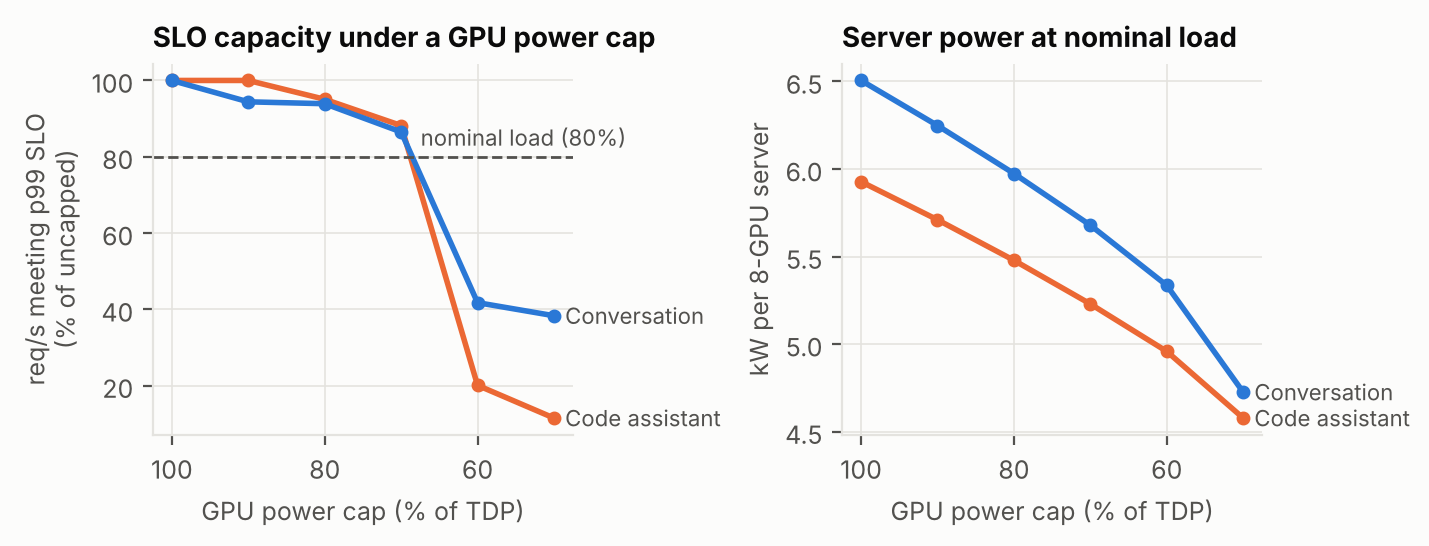
\includegraphics[width=\linewidth]{figures/fig2a_power_cap_tradeoff.png}
    \caption{Power capping an 8-GPU LLM-serving replica (conversation and code-assistant services from the Azure 2024 trace). Left: request rate that still meets the p99 SLO (TTFT 1\,s, TPOT 100\,ms) as a fraction of uncapped capacity; dashed line: nominal provisioning at 80\%. Right: server power at nominal load.}
    \label{fig:cap}
\end{figure}

\Cref{fig:week} shows one week of the resulting envelope for a 300\,MW campus. The campus draws 157.4\,MW on average (peak 201.9\,MW, load factor 0.525). Only 7.7\,MW on average, or \textbf{4.9\% of load}, can be shed within the SLO. Deferrable batch work accounts for \textbf{19.8\% of energy}, with 62.2\,MW of mean headroom. \Cref{fig:sweeps} shows that sheddable power grows from 0.8\% of load at 0.6$\times$ the default SLO to 10.2\% at 2$\times$, while the shiftable share scales with the amount of batch work (11.0\% at 25\% fill, 30.7\% at 90\% fill). Claims that a data center is ``$X$\% flexible'' therefore implicitly assume a batch share.

\begin{figure}[t]
    \centering
    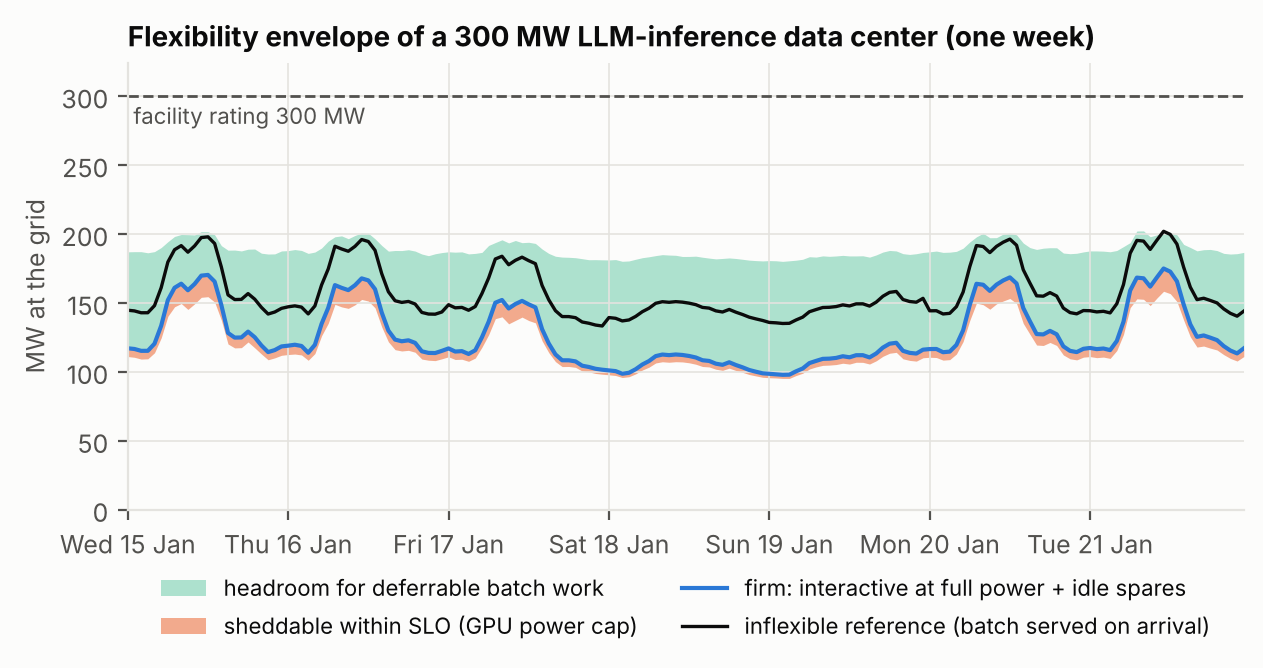
\includegraphics[width=\linewidth]{figures/fig2b_envelope_week.png}
    \caption{One week of the hourly flexibility envelope of a 300\,MW LLM-inference campus: firm power (interactive serving at full power plus idle spares), power sheddable within the SLO by GPU power capping, headroom for deferrable batch work, and the inflexible reference that serves batch work on arrival.}
    \label{fig:week}
\end{figure}

\begin{figure}[t]
    \centering
    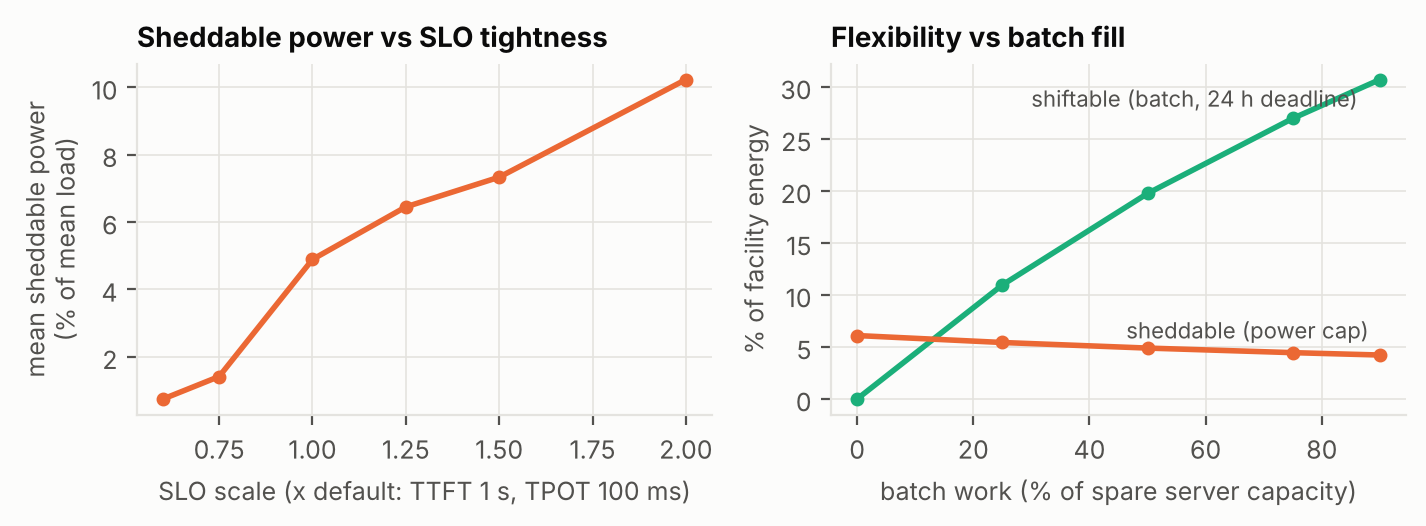
\includegraphics[width=\linewidth]{figures/fig2c_flex_sweeps.png}
    \caption{Sensitivity of the envelope. Left: mean sheddable power against SLO tightness (multiplier on both TTFT and TPOT targets). Right: shiftable (batch) and sheddable shares of facility energy against the amount of batch work.}
    \label{fig:sweeps}
\end{figure}

\subsection{Signals matter more than flexibility}
\label{sec:exp_signals}
Hosting an inflexible 300\,MW campus (1.375\,TWh/yr) adds \$24.65--34.38M/yr of generation cost and 657--1{,}111\,kt/yr of CO$_2$ at the four hostable sites. Its hosting CO$_2$ intensity ranges from 0.478\,t/MWh (bus 303) to 0.808\,t/MWh (bus 101): location alone changes the footprint by 69\%. \Cref{tab:signals} and \cref{fig:value,fig:paradox} compare steering signals that all use the same envelope.

\begin{table}[t]
    \centering
    \caption{One-year change versus an inflexible campus at the same bus, as \% of the campus's hosting impact (negative is better). Congestion cost is the cost on the network minus the cost of the same loads on a copper plate. RTS-GMLC, lines at 0.6$\times$, 300\,MW campus.}
    \label{tab:signals}
    \small
    \begin{tabular}{llrrr}
        \toprule
        Bus & Signal & $\Delta$ cost (\%) & $\Delta$ CO$_2$ (\%) & $\Delta$ congestion cost (\%) \\
        \midrule
        \multirow{4}{*}{101 (coal)} & Price (LMP) & $-2.77$ & $+0.86$ & $+0.40$ \\
         & Average CI & $-1.80$ & $0.00$ & $+0.91$ \\
         & LME & $-1.38$ & $-5.73$ & $+0.29$ \\
         & Co-optimised & $-2.78$ & $+0.88$ & $+0.39$ \\
        \midrule
        \multirow{4}{*}{122 (wind)} & Price (LMP) & $-6.79$ & $-3.39$ & $-2.01$ \\
         & Average CI & $-3.98$ & $-2.18$ & $+0.16$ \\
         & LME & $-5.26$ & $-11.90$ & $-1.85$ \\
         & Co-optimised & $-6.66$ & $-3.08$ & $-2.04$ \\
        \midrule
        \multirow{4}{*}{303 (wind pocket)} & Price (LMP) & $-8.33$ & $-3.67$ & $-3.69$ \\
         & Average CI & $-3.30$ & $-0.16$ & $+0.41$ \\
         & LME & $-6.27$ & $-12.28$ & $-3.07$ \\
         & Co-optimised & $-8.39$ & $-3.22$ & $-3.81$ \\
        \midrule
        \multirow{4}{*}{313 (load centre)} & Price (LMP) & $-3.91$ & $-2.38$ & $-0.64$ \\
         & Average CI & $-3.61$ & $-0.93$ & $-0.41$ \\
         & LME & $-2.24$ & $-9.56$ & $-0.05$ \\
         & Co-optimised & $-3.91$ & $-2.38$ & $-0.68$ \\
        \bottomrule
    \end{tabular}
\end{table}

\paragraph{The signal dominates.} With the same envelope, LME-following cuts hosting emissions by 5.73--12.28\%, while cost co-optimisation cuts them by at most 3.22\%, and at bus 101 it raises them. LME-following retains much of the cost benefit (for example, $-5.26\%$ versus $-6.66\%$ at bus 122). Following the system-average carbon intensity, the signal most carbon-aware schedulers use, is nearly ineffective (0.00 to $-2.18\%$). At bus 101 it is emissions-neutral even though it re-times about 250\,GWh of load.

\paragraph{Where the paradox appears.} At the coal-margined bus 101, price-following and co-optimisation lower cost by 2.8\% but raise emissions by 0.9\%: the ``lower cost, higher emissions'' effect of \citet{knittel2025flexible}, located in network terms. A 300\,MW campus is close to a price-taker, so price-following and co-optimisation give nearly identical results. A grid-wide \$50/t carbon price aligns the signals: at bus 313, price-following, LME-following and co-optimisation all reduce emissions by 22.34--22.45\,kt/yr relative to an inflexible campus on the same priced grid.

\paragraph{Ablation: which lever?} At bus 313, shifting batch work alone yields $-2.11\%$ cost and $-0.84\%$ CO$_2$; power capping alone yields $-1.81\%$ and $-1.53\%$; together they give $-3.91\%$ and $-2.38\%$. Capping's emissions benefit is essentially the 20.5\,GWh of energy it saves. Shift-only average-CI following \emph{raises} emissions by 0.47\%.

\paragraph{Network-blind signals can hurt reliability.} Bus 207 is served by a single line (105\,MW at 0.6$\times$) and cannot host 300\,MW: the inflexible campus causes 155.6\,GWh/yr of involuntary shedding. Co-optimisation reduces this by 55.5\,GWh (36\%), whereas average-CI and LME following, which ignore the network, increase it by 66.5 and 58.9\,GWh.

\begin{figure}[t]
    \centering
    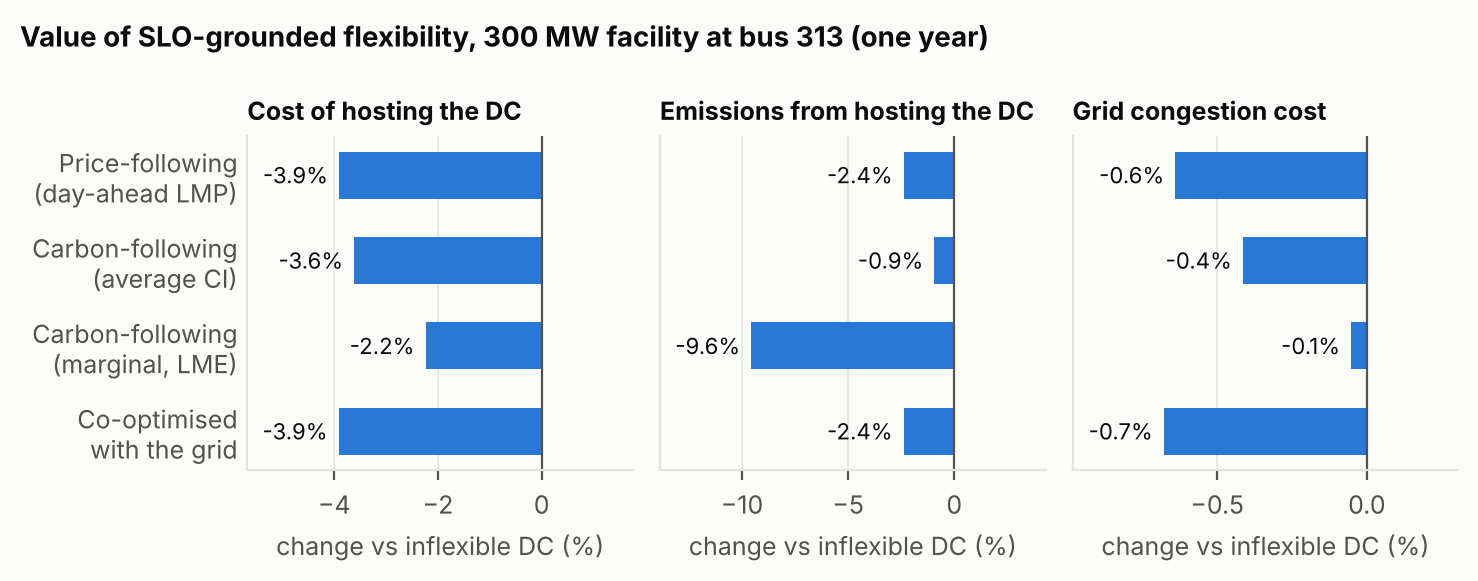
\includegraphics[width=\linewidth]{figures/fig3_value_by_mode.png}
    \caption{One-year value of the same envelope under different steering signals for a 300\,MW campus at bus 313: change against an inflexible campus in hosting cost, hosting emissions and grid congestion cost.}
    \label{fig:value}
\end{figure}

\begin{figure}[t]
    \centering
    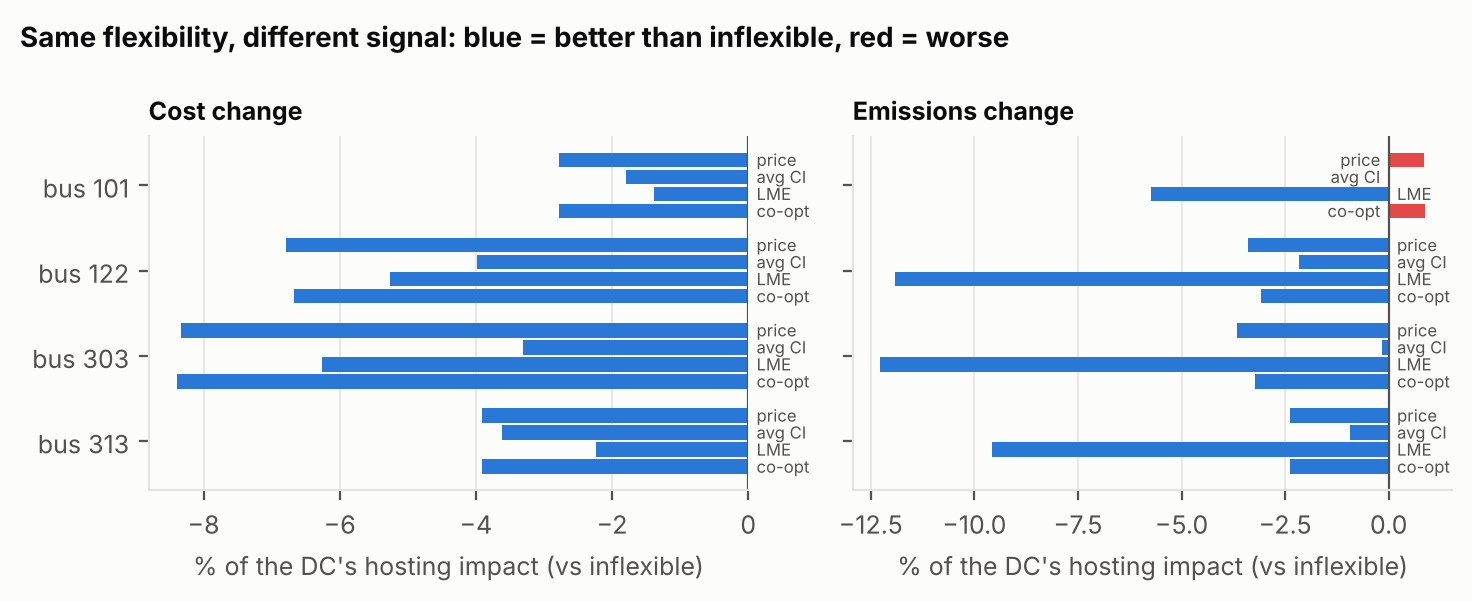
\includegraphics[width=\linewidth]{figures/fig4_signal_paradox.png}
    \caption{Same flexibility, different signal, across the four hostable buses: change in hosting cost and hosting emissions against an inflexible campus (blue: better, red: worse). Price-following and cost co-optimisation raise emissions at the coal-heavy bus 101.}
    \label{fig:paradox}
\end{figure}

\subsection{Where can a campus connect?}
\label{sec:exp_map}
\Cref{fig:map} and \cref{tab:map} report the certified map for all 73 buses. SLO-feasible flexibility enlarges the set of hostable buses for every size: from 53 to 60 at 250\,MW, from \textbf{36 to 48 at 500\,MW}, and from 23 to 30 at 1{,}000\,MW. Summed over buses (one campus at a time), hosting capacity rises from 35.25 to \textbf{42.90\,GW (+22\%)}. Most of the gain comes from inexpensive rungs, power capping (L1) and 4\,h deferral (L2); no site requires exactly 24\,h deferral as its minimum.

\begin{figure}[t]
    \centering
    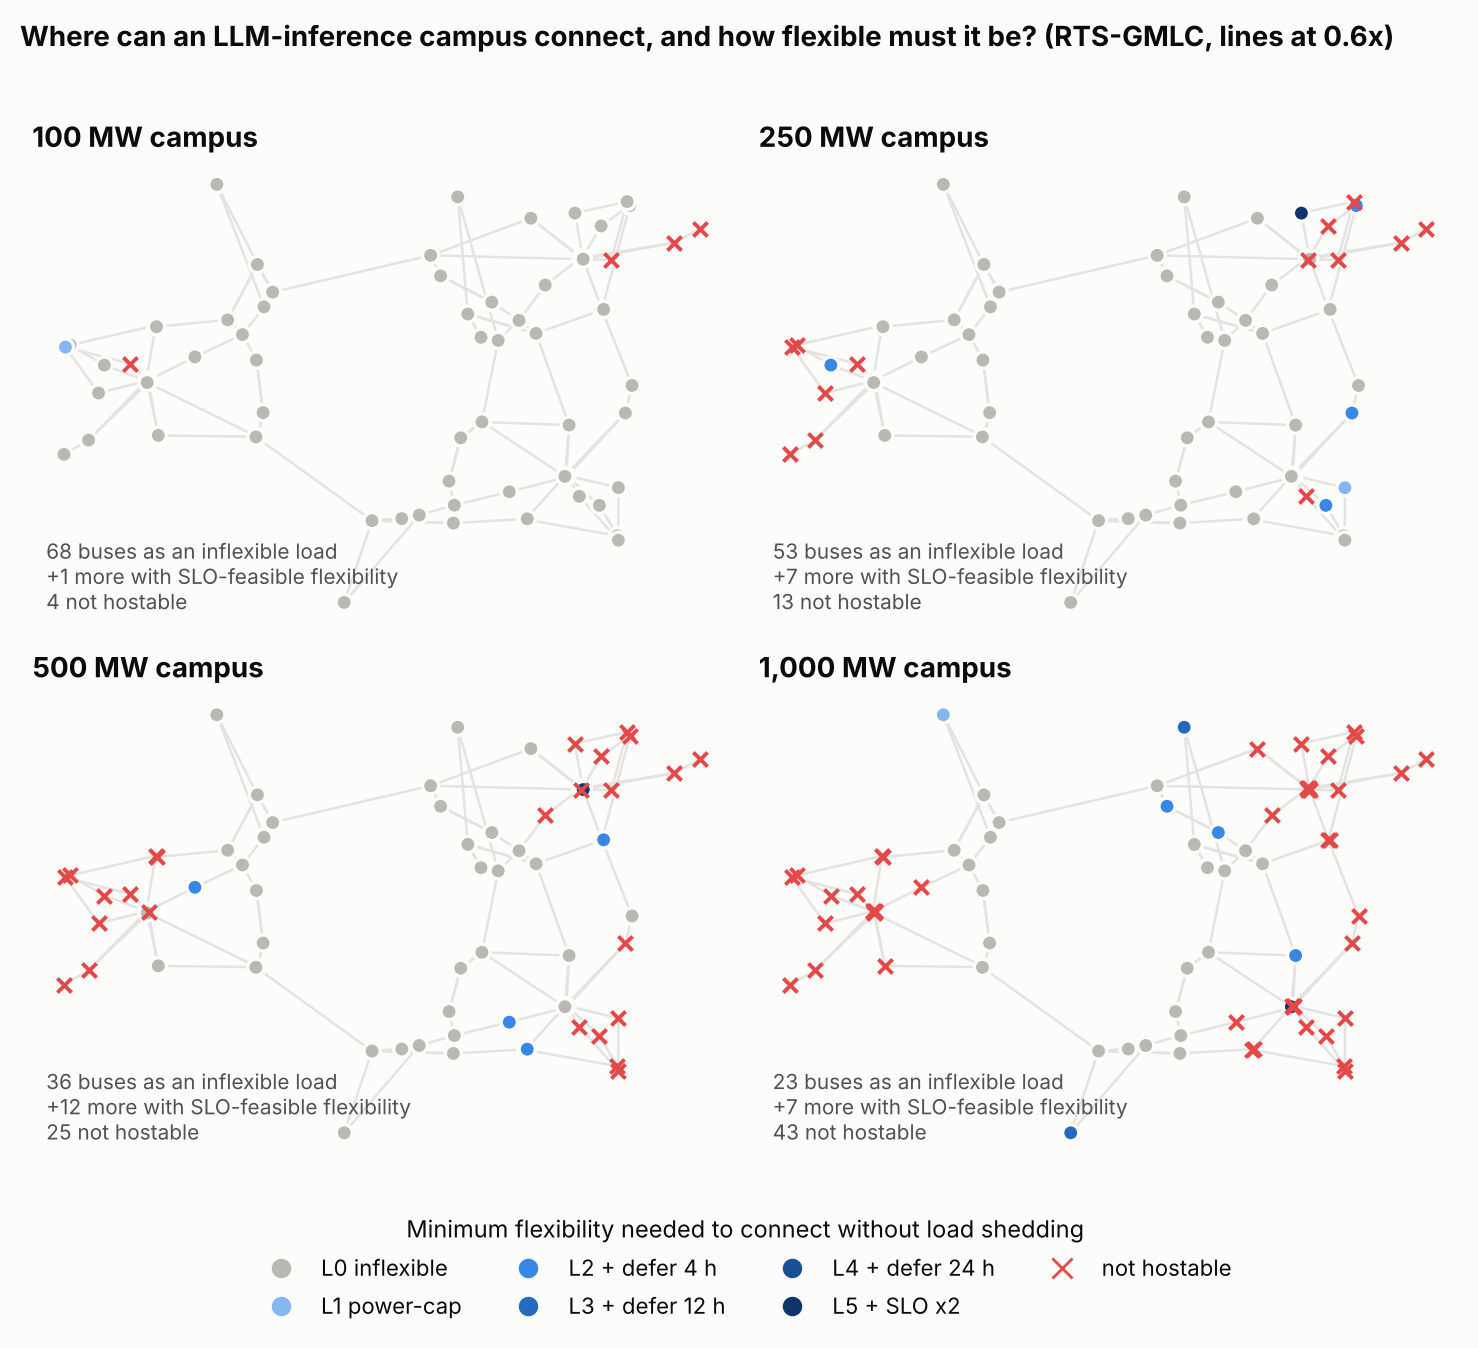
\includegraphics[width=\linewidth]{figures/fig1_flex_interconnection_map.png}
    \caption{Flexible-interconnection map on RTS-GMLC (lines at 0.6$\times$). For campuses of 100, 250, 500 and 1,000\,MW, each bus shows the minimum rung of the SLO-feasible flexibility ladder at which the campus connects with no involuntary load shedding and no missed batch deadline (gray: inflexible suffices; blue ramp: power capping, 4/12/24\,h deferral, relaxed-SLO capping; red cross: not hostable). Flexible entries are verified over all 365 days.}
    \label{fig:map}
\end{figure}

\begin{table}[t]
    \centering
    \caption{Number of buses (of 73) by certified minimum flexibility level.}
    \label{tab:map}
    \small
    \begin{tabular}{lrrrr}
        \toprule
        Minimum level & 100\,MW & 250\,MW & 500\,MW & 1{,}000\,MW \\
        \midrule
        L0 inflexible & 68 & 53 & 36 & 23 \\
        L1 power cap & 1 & 1 & 2 & 1 \\
        L2 defer 4\,h & 0 & 5 & 8 & 3 \\
        L3 defer 12\,h & 0 & 0 & 0 & 2 \\
        L5 relaxed-SLO capping & 0 & 1 & 2 & 1 \\
        Not hostable & 4 & 13 & 25 & 43 \\
        \bottomrule
    \end{tabular}
\end{table}

\paragraph{Why full-year verification is necessary.} Stage 2 raised 10 of the 30 flexible entries found on stress days. Full-year spot checks explain why. At bus 101 with 500\,MW, the stage-1 level L2 passes every stress day but fails on 2 other days (10.8\,MWh of shedding). At bus 122 with 1{,}000\,MW, L2 misses batch deadlines on 4 days. Doubling the stress days from 2 to 4 per month changed only 1 of 292 entries: stress days chosen from system load miss days that are stressful \emph{locally}. In every spot check, the level below the stage-1 answer fails on real days, confirming that stage 1 yields exact lower bounds. All 9 sampled inflexible (L0) entries held on all 365 days.

\subsection{Can hard-constraint learners solve the joint problem?}
\label{sec:exp_solvers}
The 24\,h joint problem at bus 313 has 5{,}496 decision variables after completion; HiGHS solves it in 243.8\,ms. We train on 1{,}168 HiGHS-labelled instances and test on 296 held-out days and on 74 out-of-distribution instances (a 600\,MW campus at 90\% batch fill). \Cref{tab:solvers} and \cref{fig:solvers} show the results.

\begin{table}[t]
    \centering
    \caption{Solver benchmark on held-out days (test) and out-of-distribution instances (OOD, 600\,MW). Exact methods were timed one instance at a time; learned methods were batched on 4 CPU threads.}
    \label{tab:solvers}
    \small
    \begin{tabular}{lrrrrr}
        \toprule
        Method & ms/inst. & Speed-up & Gap (\%) & Max viol. (MW) & OOD speed-up \\
        \midrule
        HiGHS, full LP & 243.83 & 1.00 & 0 & 0 & 1.00 \\
        Constraint generation & 111.02 & 2.20 & 0 & 0 & 2.08 \\
        Frequency screening + CG & 75.86 & 3.21 & 0 & 0 & 2.76 \\
        Learned screening + CG & 93.76 & 2.60 & 0 & 0 & 2.30 \\
        Oracle screening (bound) & 35.22 & 6.92 & 0 & 0 & 6.95 \\
        \midrule
        DC3-style & 11.35 & 21.48 & 211.07 & 178.36 & 30.13 \\
        Predict--correct--project & 7.23 & 33.73 & 11{,}268.15 & 0 & 31.02 \\
        Gauge map & 0.80 & 306.15 & 2{,}566.15 & 0 & 223.87 \\
        \bottomrule
    \end{tabular}
\end{table}

\begin{figure}[t]
    \centering
    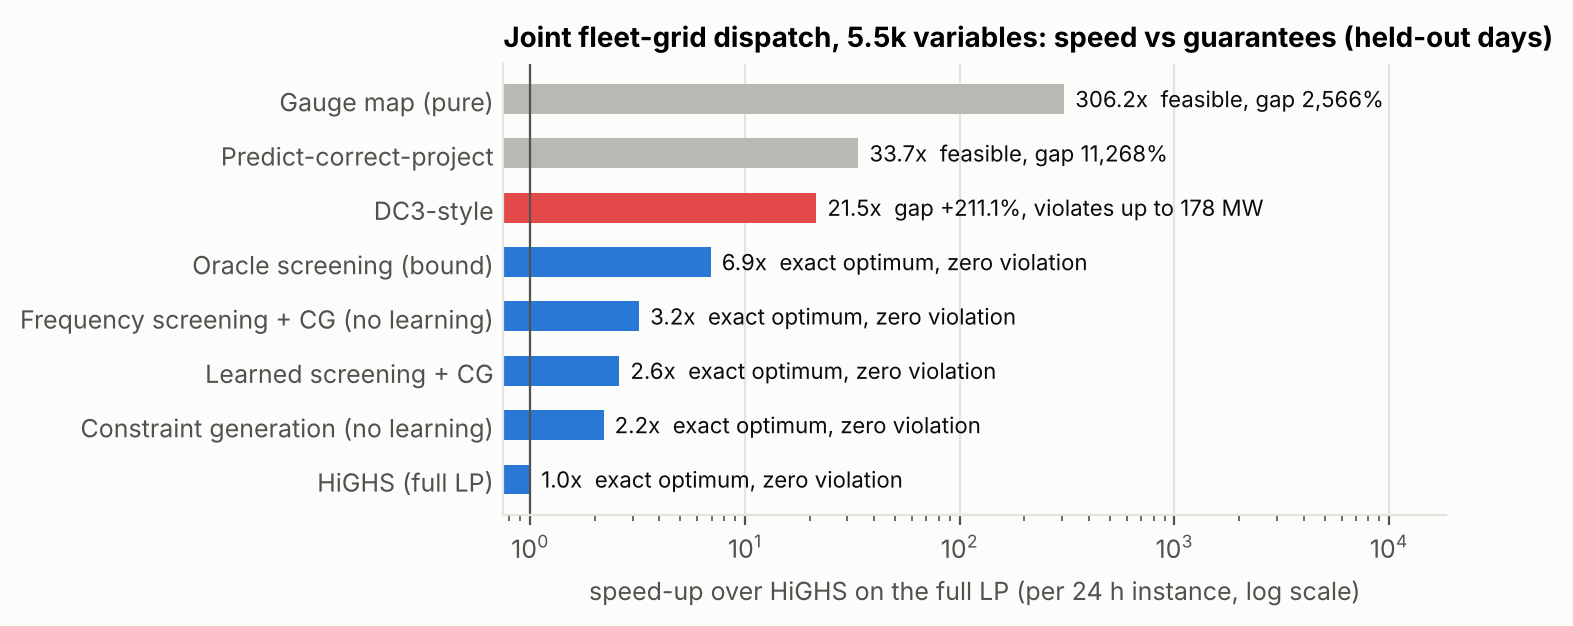
\includegraphics[width=\linewidth]{figures/fig5_solver_benchmark.png}
    \caption{Speed versus guarantees for the 24\,h joint fleet--grid dispatch (5.5k variables) on held-out days. Exact screening with constraint generation reaches the exact optimum with zero violations; end-to-end constraint-enforcing learners are either infeasible (DC3-style) or feasible but far from optimal (gauge map, predict--correct--project).}
    \label{fig:solvers}
\end{figure}

\paragraph{The interior-anchor barrier.} Completing equalities is easy if done right. A single-pivot completion concentrates the prediction error of about 5{,}000 variables on one bus (about 2{,}000\,MW), whereas a distributed slack keeps the slack within 0.15. Inequalities are the obstacle. A strictly interior anchor exists in closed form for 100\% of instances, but in an OPF whose only slack is load shedding, \emph{every} strictly interior point sheds load at every bus. Gauge maps and ray projections, which guarantee feasibility by retracting toward such an anchor, therefore pay VOLL on the retraction. Their outputs are always feasible, yet their mean optimality gaps are 2{,}566\% and 11{,}268\%. DC3-style correction stays near the optimum in cost but violates line limits by up to 178\,MW (523\,MW out of distribution). FSNet-style L-BFGS feasibility seeking stalls at 13--40\,MW of violation and takes 160--800\,ms per instance, slower than HiGHS.

\paragraph{Exact screening wins.} Solving with only predicted-binding line limits and adding back any violated limit is optimal and feasible by construction. A simple frequency screen (3.21$\times$, 1.19 rounds) beats our learned screen (2.60$\times$); the learned screen reaches only 77\% recall on unseen days, and its flagged rows are a subset of the frequency screen's. Perfect screening would allow 6.92$\times$. Every point of the interconnection map in \cref{sec:exp_map} was computed with exact screened solves.
%%%%%%%%% EXPERIMENTS %%%%%%%%%

\section{Conclusion}
\label{sec:conclusion}
%%%%%%%%% CONCLUSION %%%%%%%%%
We derived the grid-facing flexibility of LLM inference fleets from serving physics and latency SLOs, and evaluated it inside a year of network-constrained dispatch. Three findings stand out. Interactive serving is barely flexible; flexibility comes from deferrable batch work. Under transmission constraints, the signal that steers flexibility matters more than its amount: locational marginal emissions cut hosting emissions 3--4$\times$ more than cost co-optimisation, and price-following raises emissions where coal is on the margin. Modest SLO-feasible flexibility raises the hosting capacity of the test system by 22\%, and the corresponding interconnection map can be certified exactly. On the solver side, interior-point-based guarantees fail on OPF with load-shedding slack, which points to a concrete open problem: learning low-cost interior anchors, or anchor-free certificates, for such problem families.

\paragraph{Limitations.} Our study uses a single test system (RTS-GMLC) with derated lines, evaluates one campus at a time, assumes perfect day-ahead foresight, omits unit commitment, and relies partly on assumed fleet parameters that have not yet been swept. It is a simulation study, not a deployment. Extending the map to simultaneous multi-campus hosting and to larger systems are natural next steps.
%%%%%%%%% CONCLUSION %%%%%%%%%

%%%%%%%%% REFERENCES %%%%%%%%%
\bibliography{references}
\bibliographystyle{iclr2025_conference}
%%%%%%%%% REFERENCES %%%%%%%%%

\end{document}
